\chapter{Introduction}\label{sec:intro}

\paragraph{What is the use of that?}FA$\mu$ST is a C++ toolbox, useful to decompose a given dense matrix into a product of sparse matrices in order to reduce its computational complexity (both for storage and manipulation). In Figure \ref{fig:presentation}, the matrix \textbf{A} represents the dense matrix and $\mathbf{S_j}$ correspond to the sparse matrices as $\mathbf{A}=\prod_{j=1}^J\mathbf{S_j}$.

\begin{figure}[H] %%[!htbp]
\centering
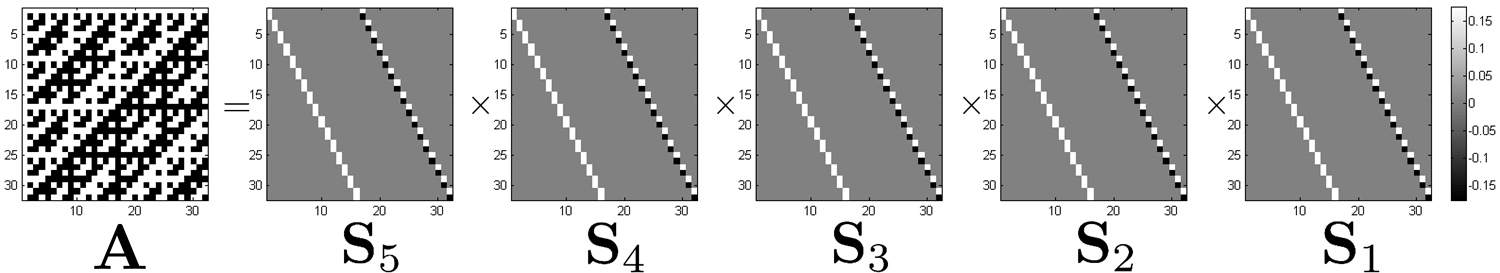
\includegraphics[scale=0.5]{images/hadamard32_bw.pdf}
\caption{Brief presentation of FA$\mu$ST}
\label{fig:presentation}
\end{figure}

FA$\mu$ST can be used to speed up iterative algorithms commonly used for solving high dimensional linear inverse problems. The algorithms implemented in the toolbox are described in details by Le Magoarou.\cite{LeMagoarou2016}.
The FA$\mu$ST toolbox is delivered with a Matlab wrapper. 
For more information on the FA$\mu$ST project, please visit the website of the project: \url{http://faust.gforge.inria.fr}.

%\paragraph{Brief description:} 
%$A=\prod_{j=1}^J S_j$.

%Valid Installation: Platforms, Compiler and IDE
\paragraph{Which type of Platform and Compiler for the installation?} 
The Figure \ref{fig:recapInstall} summarizes the tested configurations of the installation of the FA$\mu$ST toolbox following the type of platform (Linux, Mac or Windows), compiler, version of Matlab and the type of Integrate Development Environment (IDE).\\
Choose among this Figure \ref{fig:recapInstall} the adapted platform and IDE following your system and refer to the corresponding Install Chapter. Authors suggest the installation using the GCC or Clang compiler directly from a command terminal because it is more simple and requires fewer externals components. 

\begin{figure}[H] %%[!htbp]
\centering
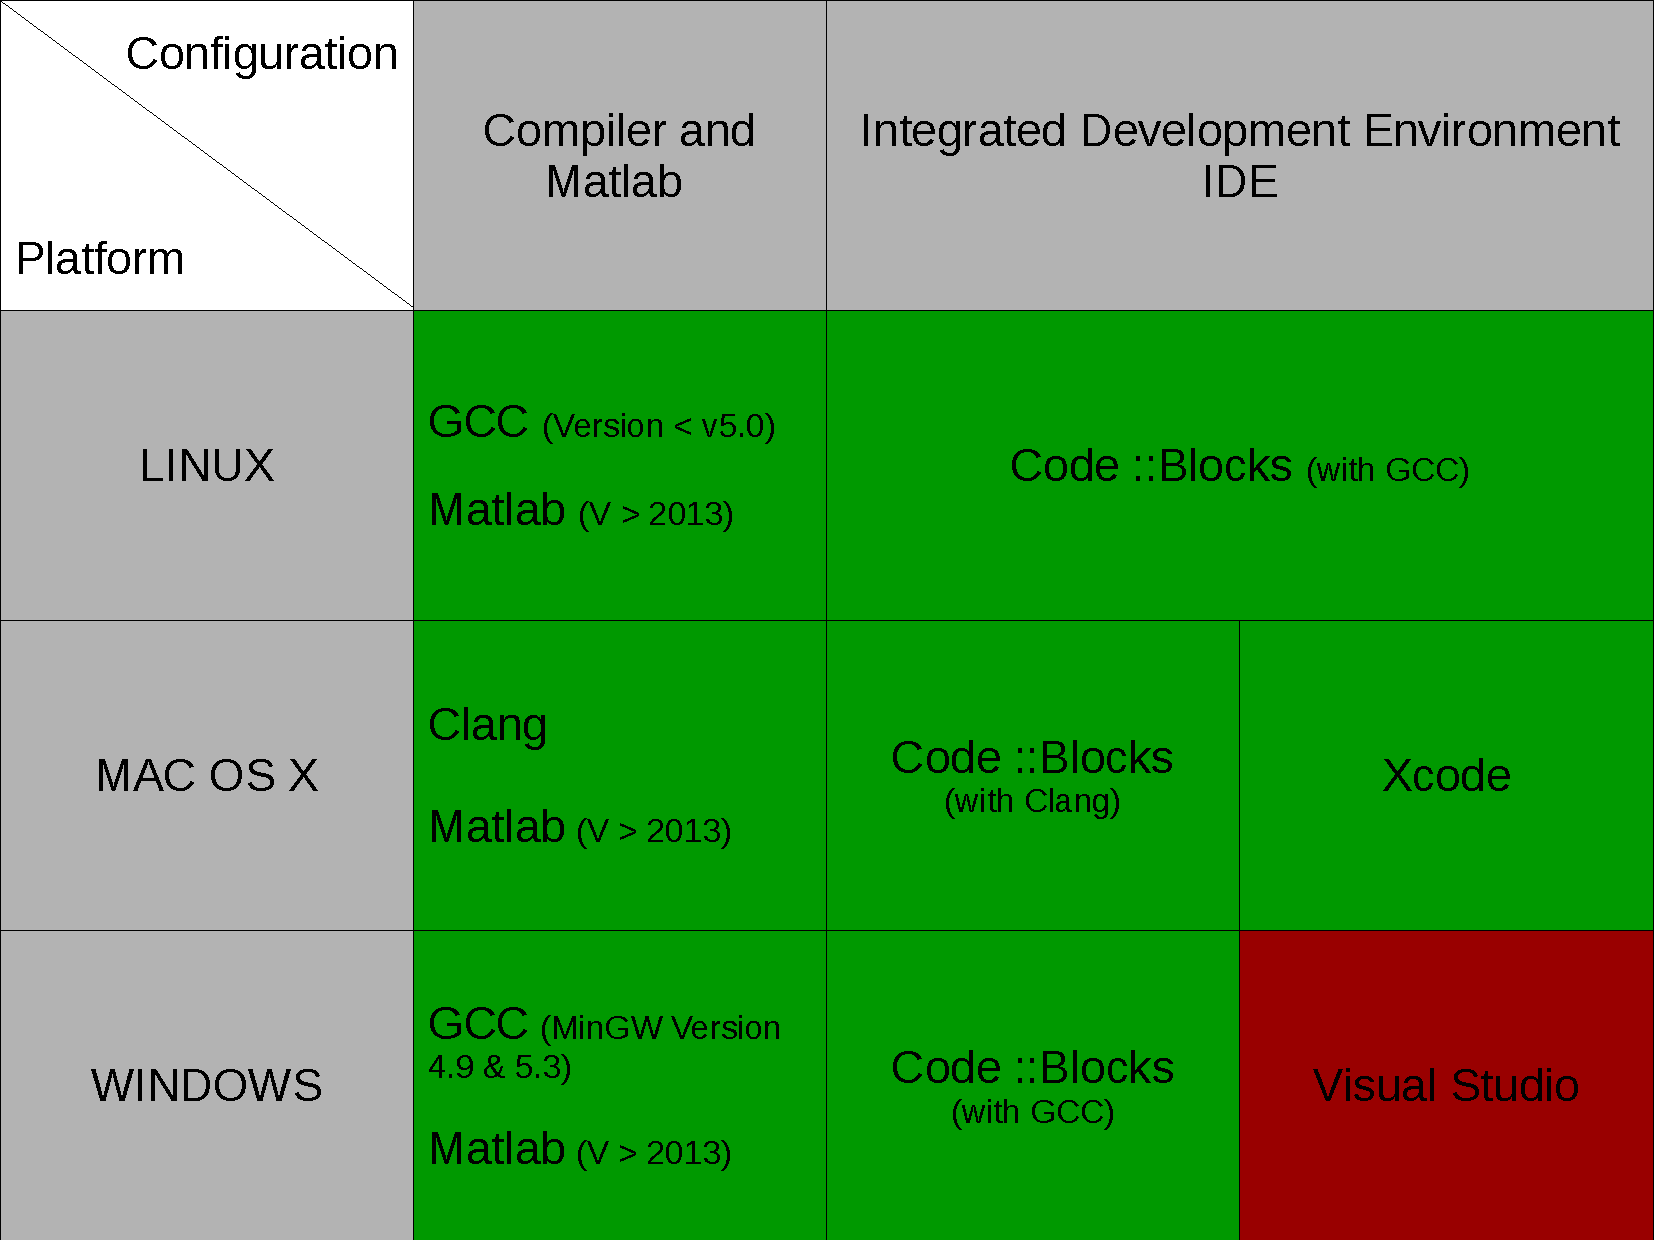
\includegraphics[scale=0.4]{images/recapInstall.pdf}
\caption{Checked Installation: Platforms and IDE}
\label{fig:recapInstall}
\end{figure}

\paragraph{How FA$\mu$ST is structured?}
The Figure \ref{fig:faustStructure} presents a brief structure of the FA$\mu$ST toolbox. The principal C++ library called "libfaust" includes two components: the "Factorization algorithms" is used to generate a FA$\mu$ST core from a dense matrix and the "FA$\mu$ST matrix multiplication" provides the linear operator to manipulate your data. It can be employ using different types of wrappers but in the second version of FA$\mu$ST package (Version 2.0), only Matlab wrapper is provided. 


\begin{figure}[H] %%[!htbp]
\centering
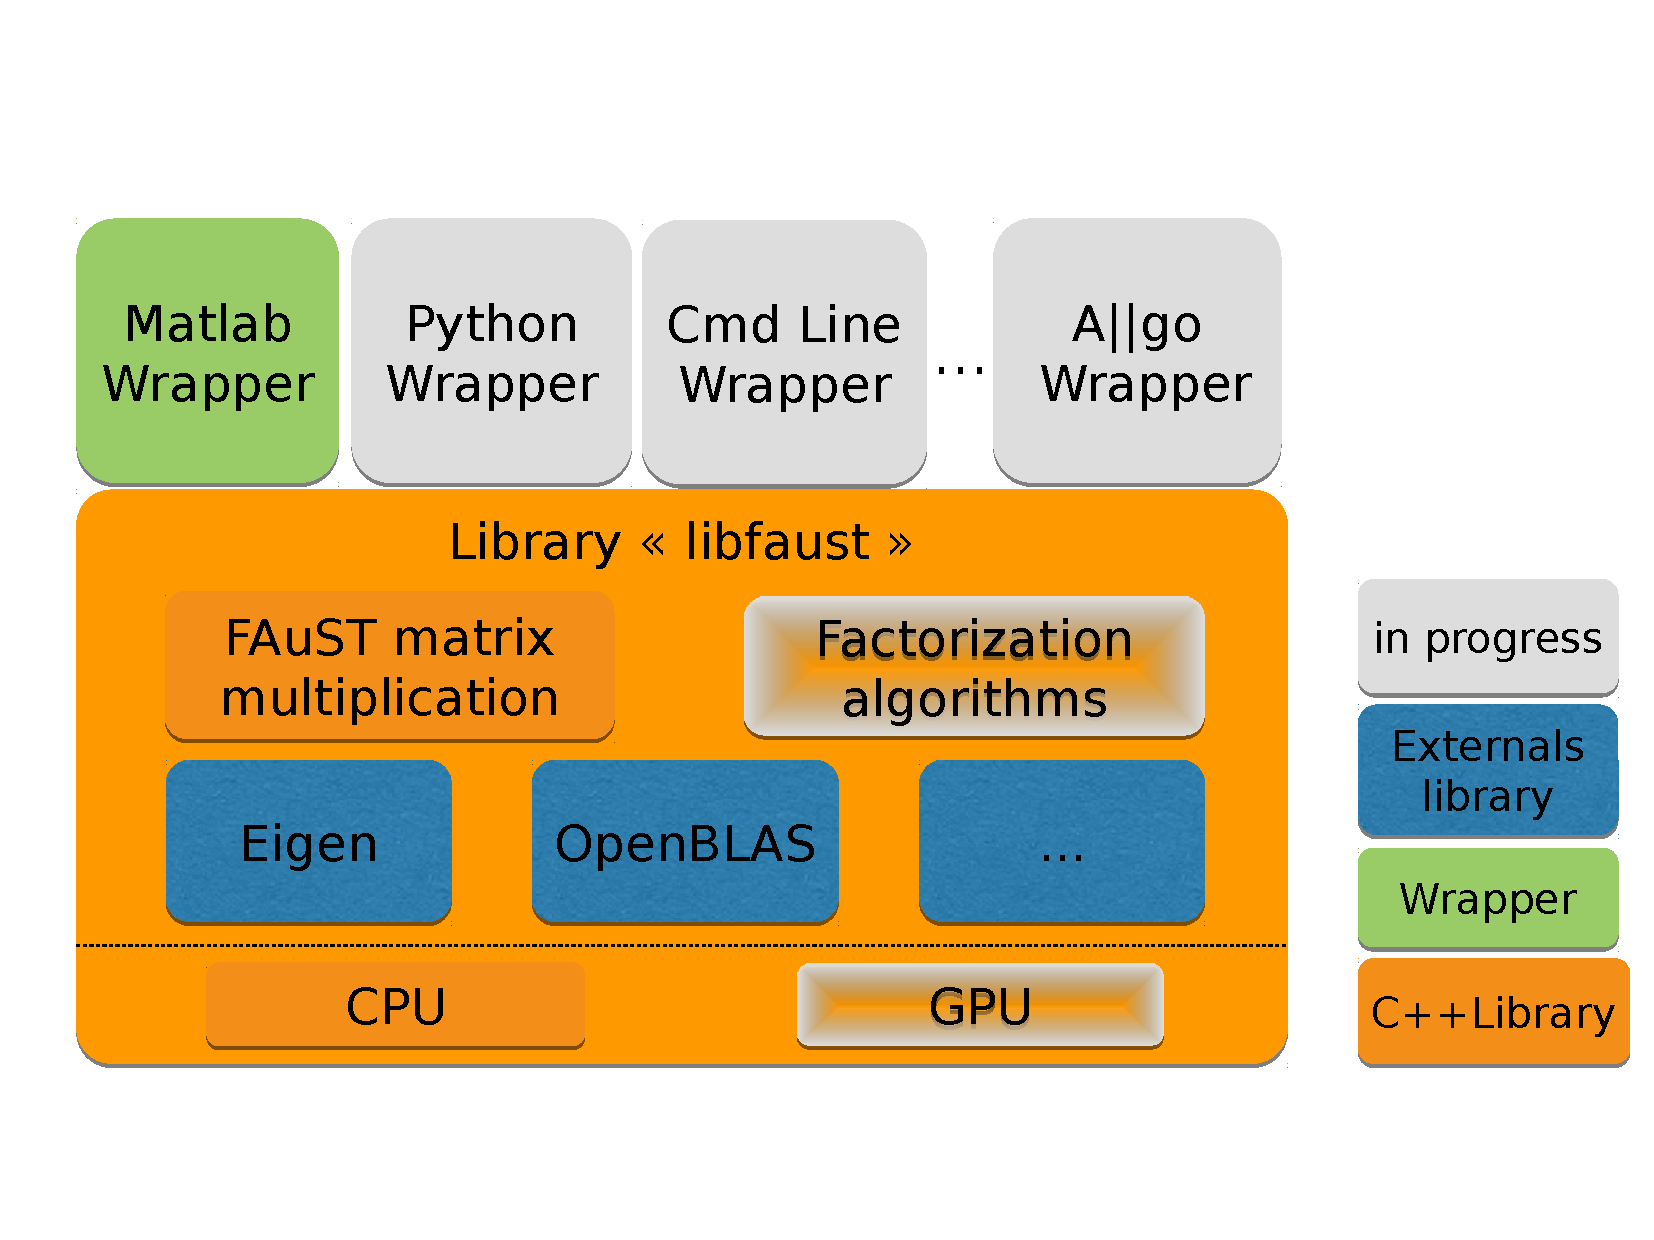
\includegraphics[scale=0.45,trim = 0cm 5cm 0cm 4cm, clip]{images/FaustStructure.pdf}
\caption{Brief structure of FA$\mu$ST version 2.0.0}
\label{fig:faustStructure}
\end{figure}

\paragraph{Known issues}
\begin{enumerate}
\item The installation on Windows Platform using Visual Studio IDE has been tested but there is compilation problems depending on the version of your Windows and your Visual Studio. \textbf{This install configuration is not guaranteed} but you can try and report any problem and/or suggestion on install-list of FA$\mu$ST project on \url{http://lists.gforge.inria.fr/pipermail/faust-install/}. 
 
\item The use of the \textbf{mex function} from Matlab requires that you have a third-party compiler installed on your system. Warning: Following your version of Matlab (2016a in our case) mex function only supports up to GCC 4.7 (see \url{http://fr.mathworks.com/support/compilers/R2016a/index.html?sec=glnxa64} for more detail).

\item The "Factorization algorithms" module represented on Figure \ref{fig:faustStructure} is actually in progress (see Section).

\end{enumerate}


\paragraph{Organization:}Chapter \ref{sec:InstallUnix} explains how to install the library FA$\mu$ST for UNIX (including Linux and Mac OS X) platform  and Chapter \ref{sec:WinInstall} corresponds to the Windows installation. Chapter \ref{sec:firstUse} shows quickly how to use this library and gives an example of application. Finally, a "working progress" part is given Chapter \ref{sec:WorkingProgress} to review the current and future work. 

\paragraph{License:}Copyright (2016) Luc Le Magoarou, Remi Gribonval INRIA Rennes, FRANCE \\
The FA$\mu$ST Toolbox is distributed under the terms of the GNU Affero General Public License. This program is free software: you can redistribute it and/or modify it under the terms of the GNU Affero General Public License as published by the Free Software Foundation. This program is distributed in the hope that it will be useful, but WITHOUT ANY WARRANTY; without even the implied warranty of MERCHANTABILITY or FITNESS FOR A PARTICULAR PURPOSE.  See the GNU Affero General Public License for more details. You should have received a copy of the GNU Affero General Public License along with this program.  If not, see \url{http://www.gnu.org/licenses/}.
